\subsection{Molle e Forza Elastica}
\begin{center}
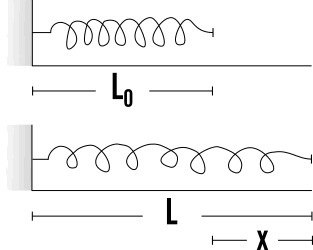
\includegraphics[width=0.4 \linewidth]{Dinamica/forza-elastica.png} 
\end{center}
\begin{gather*}
    \text{Lunghezza della molla a riposo: } L_0 \\
    \text{Elongazione: } x = L - L_0 \\
    \text{Legge di Hooke(Forza Elastica): } F_e = -k x 
\end{gather*}
\subsubsection{Oscillazione - Moto di una molla}
\textbf{Nota bene: } una molla quando viene rilasciata oscilla con un \textbf{Moto Armonico Semplice}.
\begin{gather*}
    \text{Frequenza angolare: } \omega = \sqrt{\frac{k}{m}} = \frac{2 \pi}{T} \\
    \text{Periodo: } T = 2 \pi \sqrt{\frac{m}{k}} = \frac{2 \pi}{\omega} \\
    \text{Costante elastica: } k = \frac{1}{m} (\frac{2 \pi}{T})^2 = m \omega^2 \\
    \text{Frequenza: } f = \frac{1}{t} = \frac{\omega}{2 \pi} \\
    \text{Ampiezza Oscillazione: } A = \frac{x}{\cos (\omega T)} \\
    \text{Elongazione: } x = A \cos (\omega T) \\
    \text{Velocità oscillazione: } v = A \omega
\end{gather*}